\chapter{使用案例}

\begin{figure*}[ht]
    \centering
    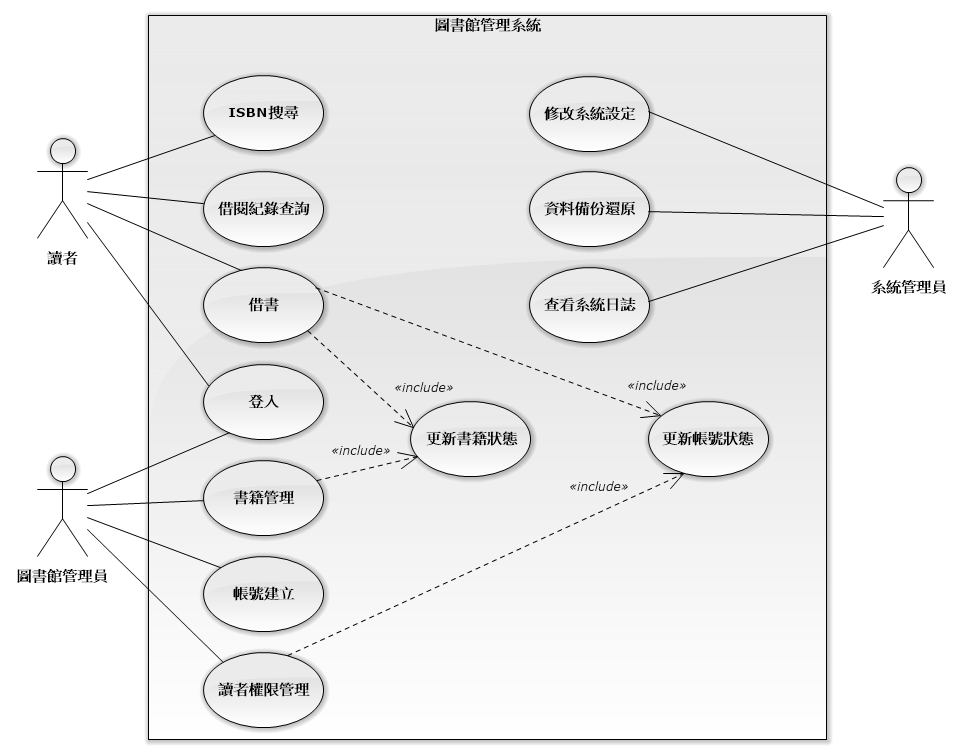
\includegraphics[width=\linewidth]{image/使用案例.png}
    \captionsetup{justification=centering}
    \caption{完整使用案例圖}
\end{figure*}

在此系統中,使用者與管理員透過登入、搜尋、借還及帳號書籍管理功能互動。

\clearpage

\section{使用者角色}

\begin{figure*}[ht]
    \centering
    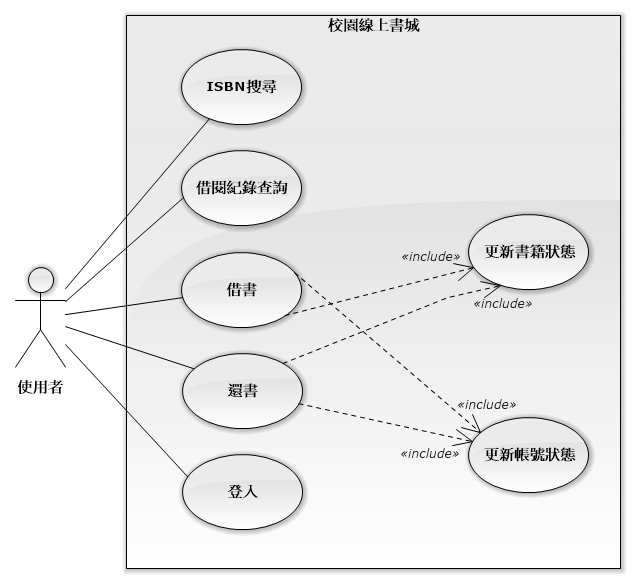
\includegraphics[width=\linewidth]{image/使用案例:使用者.png}
    \captionsetup{justification=centering}
    \caption{使用者角色的使用案例圖}
\end{figure*}

在此系統中,使用者的使用過程包含以下幾個步驟:
\begin{enumerate}
    \item 登入系統:使用者輸入校園帳號與密碼完成身份驗證,對應資料庫中「UserId」欄位。
    \item ISBN 搜尋:使用者在搜尋欄輸入ISBN,系統透過「ISBN」屬性查詢並顯示電子書詳細資訊。
    \item 借書:選擇欲借之電子書,系統建立「AccessCopy」,並執行更新書籍狀態「Amount」及更新帳號借閱次數。
    \item 還書:在到期或手動歸還時,系統更新該筆「AccessCopy」記錄狀態,並執行更新書籍狀態(Book.Amount 增加)及更新帳號狀態。
    \item 借閱紀錄查詢:使用者可查詢所有「AccessCopy」表中與自身「UserId」關聯之借閱紀錄,包含借出時間、到期時間與歸還狀態。
\end{enumerate}

\clearpage

\section{書城管理員角色}

\begin{figure*}[ht]
    \centering
    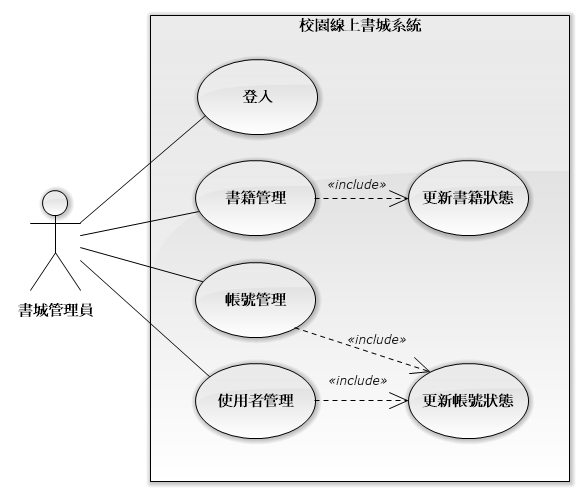
\includegraphics[width=\linewidth]{image/使用案例:書城管理員.png}
    \captionsetup{justification=centering}
    \caption{書城管理員角色的使用案例圖}
\end{figure*}

在此系統中,書城管理員的使用過程包含以下幾個步驟:
\begin{enumerate}
    \item 登入系統:管理員輸入帳號與密碼完成身份驗證,對應資料庫中「AdminId」欄位。
    \item 書籍管理:管理員可新增、修改或刪除書籍資訊,系統操作對應「Book」表中 BookId、ISBN、Amount、Publisher、ReleaseDate 等欄位,並觸發「更新書籍狀態」子流程。
    \item 帳號管理:管理員可調整使用者借閱額度或重設帳號狀態,系統更新「AccessCopy」及「User」表中的相關欄位,並執行「更新帳號狀態」子流程。
    \item 使用者管理:管理員可新增、修改或停用使用者帳號,對應「User」表中 UserId、Name、Email 等欄位,並同樣包含「更新帳號狀態」子流程。
\end{enumerate}
